\documentclass[tikz,border=2]{standalone}
%% \usepackage{amsfonts}
\usepackage{lmodern} % enhanced version of computer modern
\usepackage[T1]{fontenc} % for hyphenated characters
\usepackage{amssymb}
\usepackage{amsmath}
\usepackage{amsthm}
%
\usetikzlibrary{decorations.pathreplacing,shadows,arrows,shapes,positioning,calc,backgrounds,fit}
\newcommand{\mA}{\mathcal{A}}
\newcommand{\mB}{\mathcal{B}}
\newcommand{\mC}{\mathcal{C}}
\newcommand{\mI}{\mathcal{I}}
\newcommand{\mN}{\mathcal{N}}
\newcommand{\mP}{\mathcal{P}}
\newcommand{\mR}{\mathcal{R}}
\newcommand{\mS}{\mathcal{S}}
\newcommand{\mY}{\mathcal{Y}}
% Define the layers to draw the diagram
%
\begin{document}
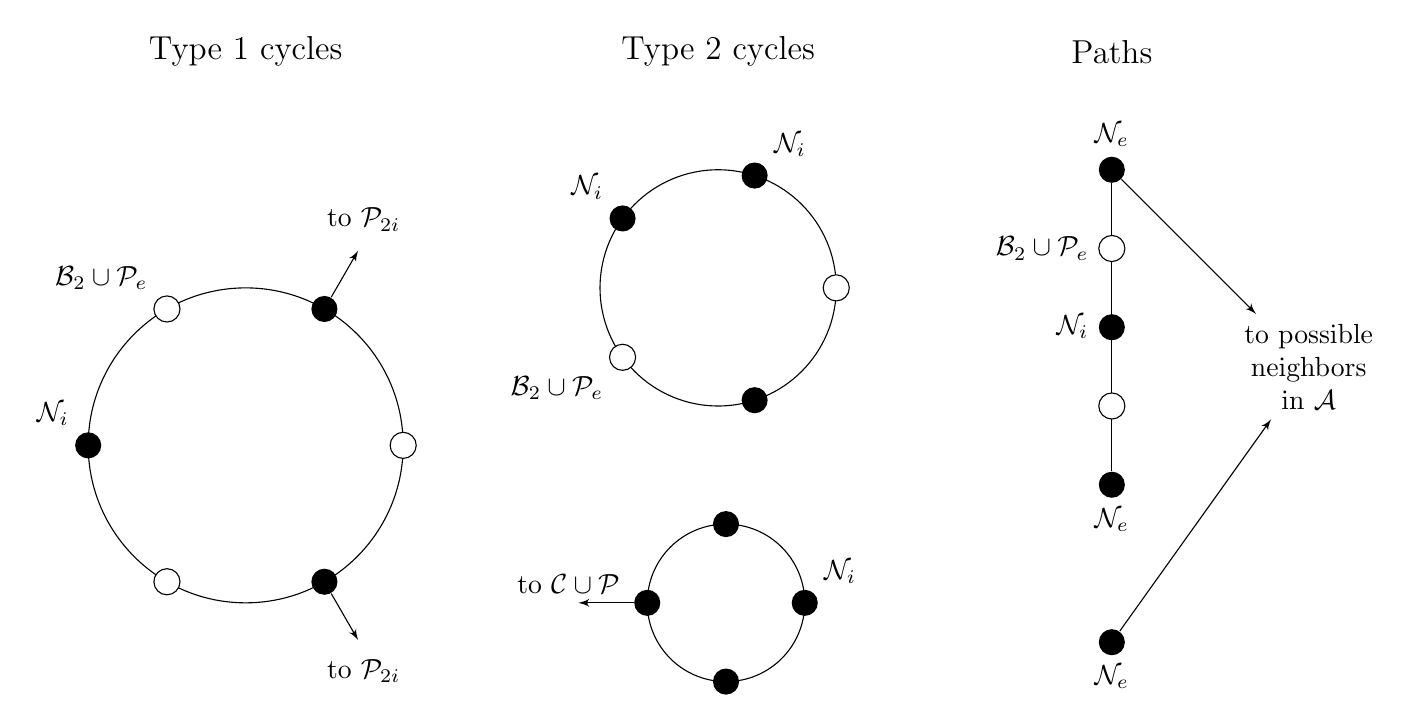
\begin{tikzpicture}
[node distance=1cm,
B2Pe/.style={draw,circle,fill=white},
N/.style={circle,fill=black},
dedge/.style={black,>=latex', shorten >=.0pt, shorten <=.0pt},
myedge/.style={thick}]
%%
%%%%%%%%%%%%%%%%%%
% Type 1 cycles
%%%%%%%%%%%%%%%%%%
\node at (0,5) {\large{Type 1 cycles}};
\def \n {6}
\def \rad {2cm}
\node[B2Pe] at ({360/\n * 0}:\rad) {};
\node[N] (Ni1) at ({360/\n * 1}:\rad) {};
\node (ref1) at ({360/\n * 1}:1.5*\rad) {};
\draw [dedge,->] (Ni1) to (ref1) node [above] {to $\mP_{2i}$};
\node[B2Pe,label=above left:$\mB_2\cup\mP_e$] at ({360/\n * 2}:\rad) {};
\node[N,label=above left:$\mN_i$] at ({360/\n * 3}:\rad) {};
\node[B2Pe] at ({360/\n * 4}:\rad) {};
\node[N] (Ni2) at ({360/\n * 5}:\rad) {};
\node (ref2) at ({360/\n * 5}:1.5*\rad) {};
\draw [dedge,->] (Ni2) to (ref2) node [below] {to $\mP_{2i}$};
%%
\begin{pgfonlayer}{background}
\draw (0,0) circle(\rad);
\end{pgfonlayer}
%%
%%%%%%%%%%%%%%%%%%
% Type 2 cycles
%%%%%%%%%%%%%%%%%%
%% cycle 1
\begin{scope}[xshift=6cm,yshift=2cm]
\node at (0,3) {\large{Type 2 cycles}};
\def \n {5}
\def \rad {1.5cm}
\node[B2Pe] at ({360/\n * 0}:\rad) {};
\node[N,label=above right:$\mN_i$] at ({360/\n * 1}:\rad) {};
\node[N,label=above left:$\mN_i$] at ({360/\n * 2}:\rad) {};
\node[B2Pe,label=below left:$\mB_2\cup\mP_e$] at ({360/\n * 3}:\rad) {};
\node[N] at ({360/\n * 4}:\rad) {};
%%
\begin{pgfonlayer}{background}
\draw (0,0) circle(\rad);
\end{pgfonlayer}
\end{scope}
%%
%% cycle 2
\begin{scope}[xshift=6.1cm,yshift=-2cm]
\def \n {4}
\def \rad {1cm}
\node[N,label=above right:$\mN_i$] at ({360/\n * 0}:\rad) {};
\node[N] at ({360/\n * 1}:\rad) {};
\node[N] (Ni3) at ({360/\n * 2}:\rad) {};
\node (ref3) at ({360/\n * 2}:2*\rad) {};
\draw [dedge,->] (Ni3) to (ref3) node [above] {to $\mC\cup\mP$};
\node[N] at ({360/\n * 3}:\rad) {};
%%
\begin{pgfonlayer}{background}
\draw (0,0) circle(\rad);
\end{pgfonlayer}
%%
\end{scope}
%%%%%%%%%%%%%%%%%%
% Paths
%%%%%%%%%%%%%%%%%%
%% path 1
\begin{scope}[xshift=11cm,yshift=-1.5cm]
\node at (0,6.5) {\large{Paths}};
\node[N,label=below:$\mN_e$] (Ne1) at (0,1) {};
\node[B2Pe] at (0,2) {};
\node[N,label=left:$\mN_i$] at (0,3) {};
\node[B2Pe,label=left:$\mB_2\cup\mP_e$] at (0,4) {};
\node[N,label=above:$\mN_e$] (Ne2) at (0,5) {};
%% path 2 (isolated node)
\node[N,label=below:$\mN_e$] (Ne3) at (0,-1) {};
%%
\begin{pgfonlayer}{background}
\draw (Ne1) -- (Ne2);
\end{pgfonlayer}
\node (A) at (2.5,2.5) {\parbox{2cm}{\centering to possible neighbors in~$\mA$}};
\draw [dedge,->] (Ne2) to (A);
\draw [dedge,->] (Ne3) to (A);
\end{scope}
%%
\end{tikzpicture}
{}
\end{document}
